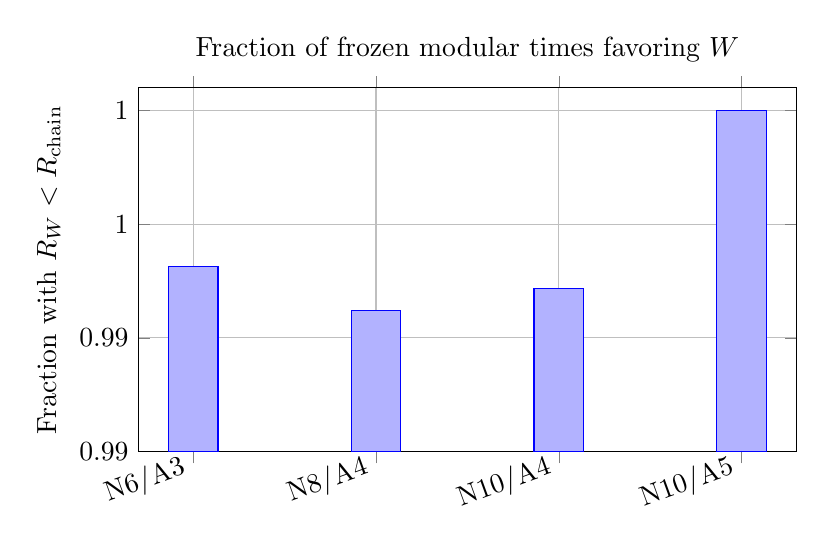
\begin{tikzpicture}
\begin{axis}[
  width=0.82\textwidth,height=6.2cm,
  ybar,bar width=18pt,
  ymin=0.985,ymax=1.001,
  ylabel={Fraction with $R_W<R_{\rm chain}$},
  symbolic x coords={N6/A3,N8/A4,N10/A4,N10/A5},
  xtick=data,
  x tick label style={rotate=20,anchor=east},
  title={Fraction of frozen modular times favoring $W$},
  grid=major
]
\addplot coordinates {(N6/A3,0.9931573803) (N8/A4,0.9912023460) (N10/A4,0.9921798631) (N10/A5,1.0)};
\end{axis}
\end{tikzpicture}
